\chapter{斯特林机组的优化}

\section{斯特林机组的排布}
\label{sec:connectionTypes}
对于单个斯特林机,斯特林机与传热流体之间的换热过程和流体的流动方向无关,这意味着改变冷热流体的流动方向并不会影响斯特林机的功率和效率。然而,对于斯特林机组,斯特林机的连接方式和流体的流动方向需要仔细考虑。它们既影响冷热流体的温度,又影响冷热流体的质量流量分布,这二者都对斯特林机的功率和效率又很大影响。
如果采用串联连接,则一方面,每个斯特林机都可以获得全部的流体流量,这有利于获得较高的输出功率;另一方面,各斯特林机的入口加热流体温度随着流动方向逐渐降低(或各斯特林机的入口冷却流体温度随着流动方向逐渐升高),这将使沿着流动方向的斯特林机的功率和效率逐渐下降。如果采用并联连接,则一方面,每个斯特林机的入口加热流体的温度都为最高值(或每个斯特林机的入口冷却流体的温度都为最低值),这有利于获得较高的输出功率;另一方面,由于每个斯特林机都分流了热流体(或冷流体)的流量,每个斯特林机的输入总能量降低,这将不利于获得较高的输出功率。如果采用顺流连接(这里的顺流和逆流是指冷热流体依次流经一列斯特林机的次序是否一致,和传统的换热器中的顺流和逆流的含义不同),则一方面,最先流经的数个斯特林机具有最大的冷热源温差,具有最大的输出功率;另一方面,最后流经的数个斯特林机具有最小的冷热源温差,具有最小的输出功率。如果采用逆流连接,则会使斯特林机组中的每个斯特林机具有接近的冷热源温差,每个斯特林机的输出功率都比较接近。对于传统的传热器,采用逆流可以降低冷热流体的传热温差,降低换热过程中产生的㶲损,并因此获得更优的换热效果。而对于斯特林机,需要增大冷热流体的温差,以提高斯特林机的输出功率和效率。
为此,分析不同斯特林机组排布方式对斯特林机组性能(包括功率和效率)的影响,并优化梯级系统中斯特林机组的排布,显得额外重要而有意义。由于斯特林机组的排列方式多种多样,既可以是串联并联,又可以是顺流逆流,还可能是四者的复杂组合。因此在分析斯特林机组的排布方式之前,需要将其进行归类。

本文依据斯特林机的性能与流体流向无关性的特点,提出了五种基本的斯特林机组排布方式,如图\ref{fig:SEA}所示。其中,第1种为并联连接,第2种为串联顺流连接,第3种为串联逆流连接,第4种为加热流体串联连接而冷却流体并联连接,第5种为加热流体并联连接而冷却流体串联连接。
所有其它的斯特林机组的连接方式都为这五种基本方式的组合。例如,图\ref{fig:SEA_eg}中斯特林机组的排布方式是第2种和第4种的组合。
%Besides, in the tradition form of solar dish system, Stirling engines are put on the focus points of the dish collectors, which can be considered as a particular case of Type 1.

\noindent \begin{figure}[htbp]
\begin{center}
	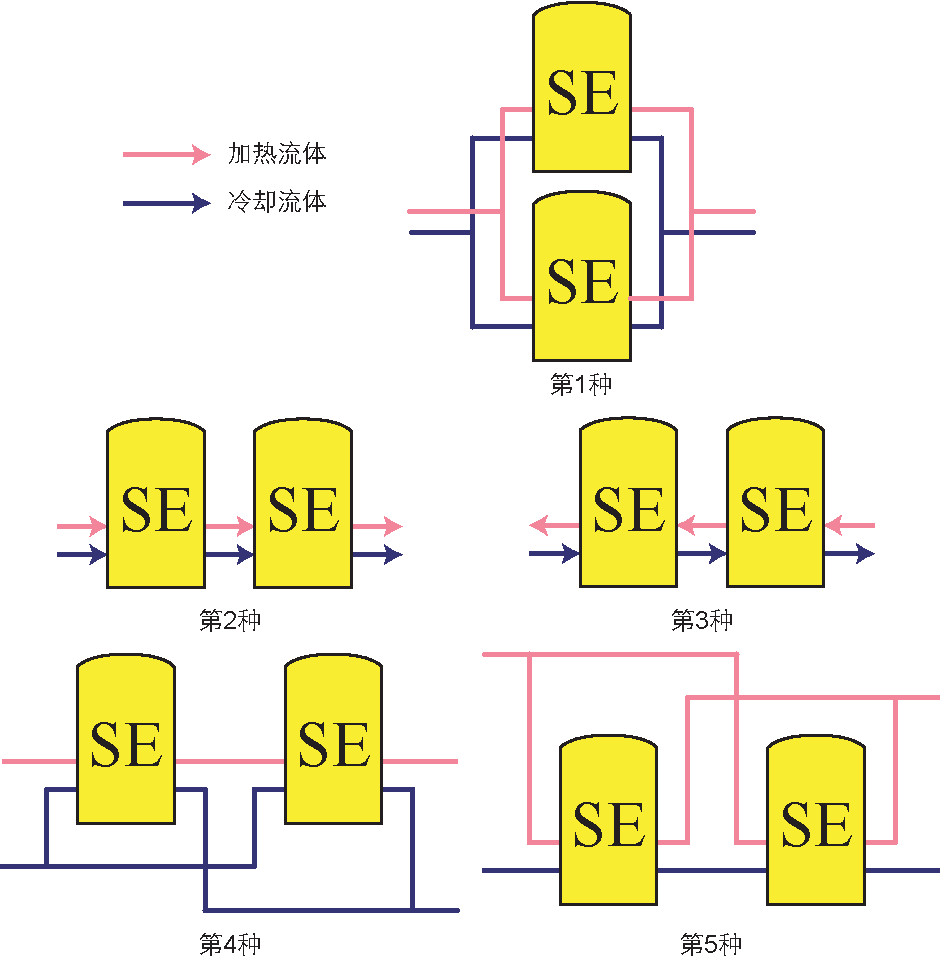
\includegraphics[width = 0.7\columnwidth]{fig/BasicSEA}
	\caption{斯特林机组的五种基本连接方式}
	\label{fig:SEA}
\end{center}
\end{figure}

\noindent \begin{figure}[htbp]
\begin{center}
	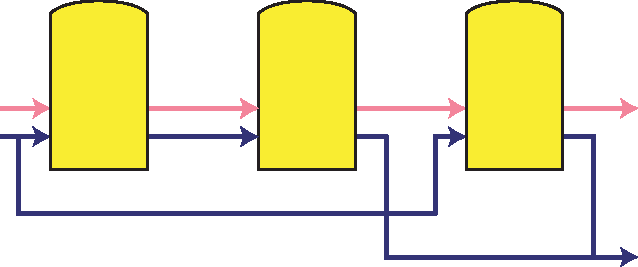
\includegraphics[width = 0.5\columnwidth]{fig/SEA_eg}
	\caption{一种斯特林机组连接方式的例子}
	\label{fig:SEA_eg}
\end{center}
\end{figure}

\section{斯特林机组的建模}

正如第\ref{sec:connectionTypes}节中所提到的,有五种基本的斯特林机组的排布方式,任何其它排布方式是这五种方式的组合。获得了这五种基本排布方式的性能计算方法,就可以得到其它排布方式的性能。

为了得到斯特林机组的性能,需要构建各斯特林机的模型,并依据斯特林机的参数对斯特林机组进行分析。为了便于分析排布方式带来的影响,选定斯特林机组中的各斯特林机具有相同的设计参数,包括转速$s_{se}$。这对于用于发电的斯特林机是个合理的假设,因为各斯特林机的输出功的频率应该保持一致。斯特林机的速度可以通过速度控制系统进行校正\cite{Hooshang2016}。为了消除其它影响,不同排布方式的冷热流体的参数也选择相同值。为了更加清楚地表明排列方式对斯特林机组性能的影响,本文选用换热后温差变化较大的空气作为传热介质。使用空气代替传统的水来给斯特林机冷却,以避免冷却斯特林过程中仅仅产生很小的温升或是导致蒸发带来的一系列不利影响。各斯特林机的设计参数如表\ref{tab:GPU3parameters}所示,斯特林机的其它参数以及冷热流体的参数如表\ref{tab:parameters}所示。如第\ref{sec:modelValidation}节中提到的,斯特林机的转速和平均有效压力分别设为25$\,\mathrm{Hz}$和5$\,\mathrm{MPa}$来使所建立的斯特林机模型获得最佳性能预测精度。

\begin{table}[htbp]
	\caption{斯特林机组模型中选用的参数}
	\begin{center}
	\begin{tabular}{cccc}
		\toprule
		参数		&	值	& 参数	&	值\\
		\midrule
		加热流体	&	空气		&	$\dot{m}_h$	&	0.4\,kg/s\\
		冷却流体	&	空气	&	$T_{i,h}$	&	1000\,K\\
		$n_{se}$	&	6	&	$p_{i,h}$	&	5$\times$10$^5$\,Pa\\
		$s_{se}$	&	25\,Hz	&	$\dot{m}_c$	&	0.4\,kg/s\\
		$p_{se}$		&	5\,MPa	&	$T_{i,c}$	&	300\,K\\
		$U_hA_h$	&	180\,W/K	&	$p_{i,c}$	&	5$\times$10$^5$\,Pa\\
		$U_cA_c$		&	180\,W/K	&&\\
		\bottomrule
	\end{tabular}
	\end{center}
	\label{tab:parameters}
\end{table}

每个斯特林机组都有两股流体,每股流体都有串联流动和并联流动两种形式,如图\ref{fig:SEA}所示。
对于串联流动,每个斯特林机的流体质量流量均为$\dot{m}$,从流体流动的方向看,对于第$x$个斯特林机($2\leqslant{}x\leqslant{}n_{se}$),
\begin{equation}
	T_{i,x} = T_{o,x-1}
	\label{Eq:T_serial}
\end{equation}
对于并联流动,每个斯特林机的流体质量流量均为$\dot{m}/n_{se}$,对于第$x$个斯特林机($2\leqslant{}x\leqslant{}n_{se}$),
\begin{equation}
	T_{i,x} = T_{i,h}
	\label{Eq:T_parallel}
\end{equation}

依据第\ref{sec:StirlingEngineModel}节中的方程及方程(\ref{Eq:T_serial})-(\ref{Eq:T_parallel}),知道了冷热流体的属性就可以求解各个斯特林机的功率(方程(\ref{Eq:P}))和效率(方程(\ref{Eq:eta}))。斯特林机组的功率和效率可以由各斯特林机的功率和热流体的流入流出参数获得。

\begin{equation}
	P_{sea} = \sum_{x = 1}^{n_{se}}P_{se,x}
\end{equation}
\begin{equation}
	\eta_{sea} = \dfrac{P_{sea}}{\dot{m}_1(h_{1o} - h_{1i})}
\end{equation}

系统以MATLAB作为建模工具,使用CoolProp提供的物性参数来进行计算分析,建立斯特林机组的模型。以前文提出的斯特林机参数和流体参数为基础,建立了五种基本斯特林机组排布方式的模型。为了比较各排布方式的性能,以几个参数为变量,研究了不同排布方式下斯特林机组在各种条件下的性能参数。

\noindent \begin{figure}[htbp]
\begin{center}
	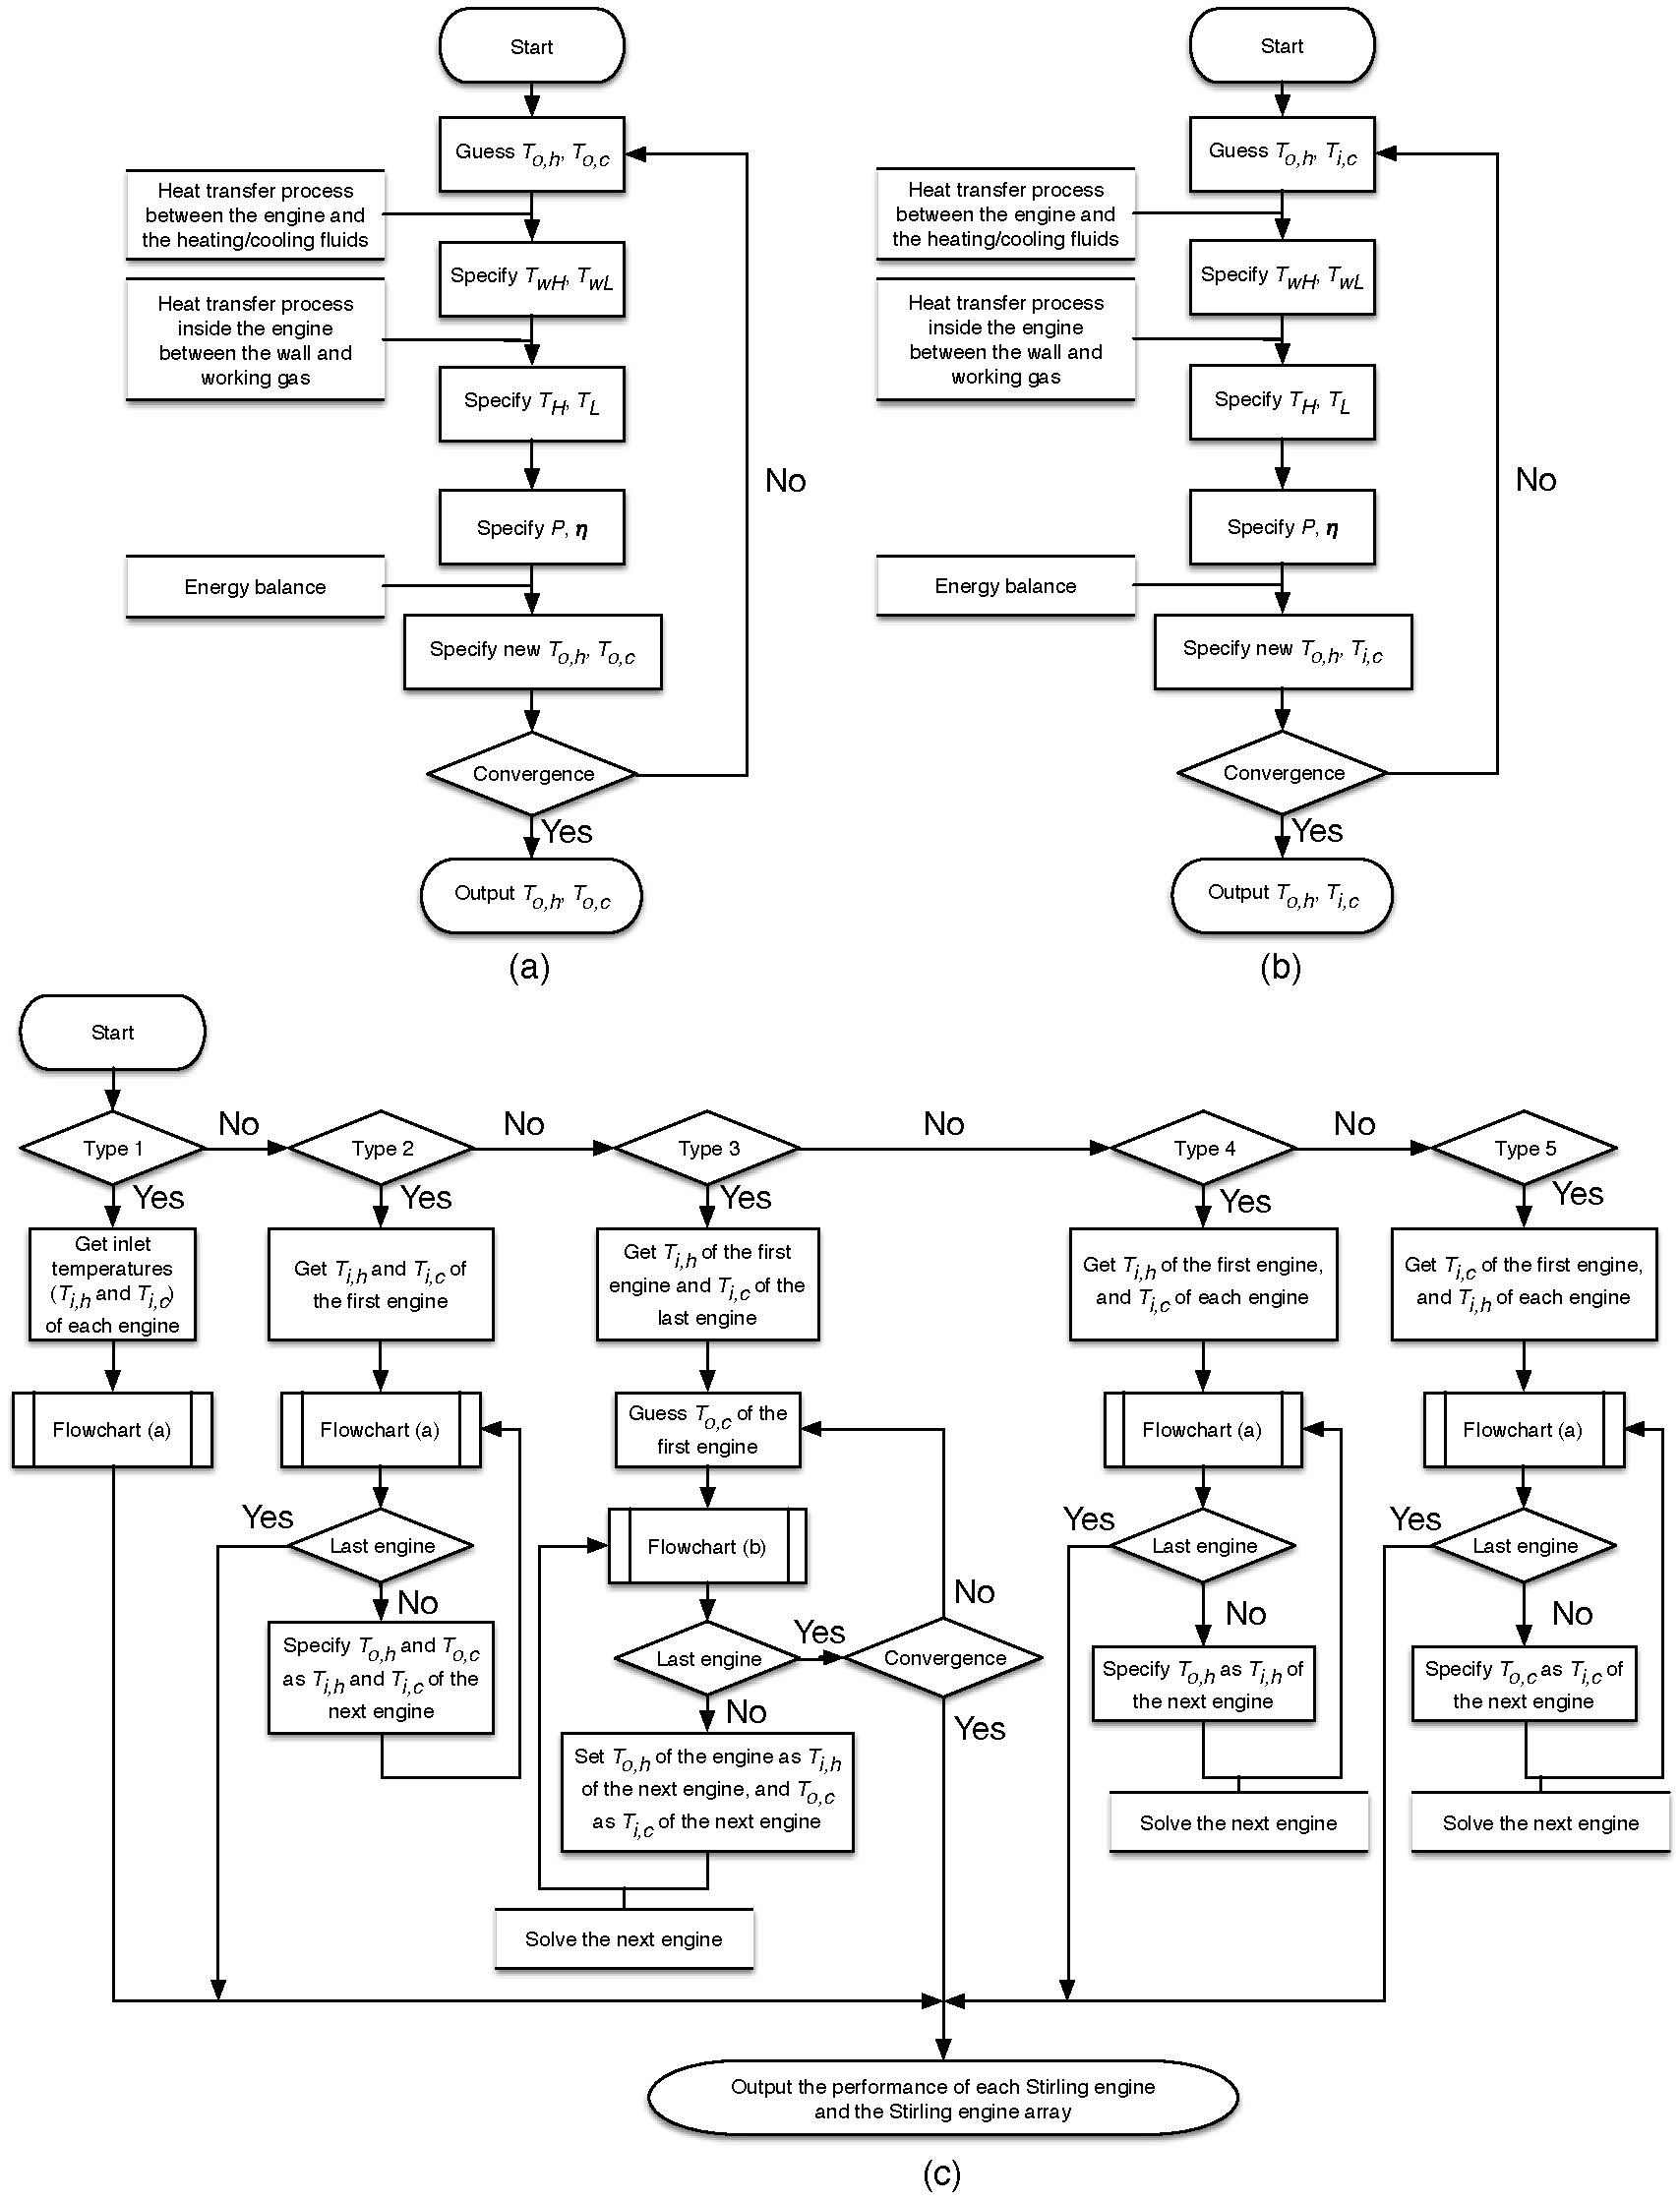
\includegraphics[width = 1.0\columnwidth]{fig/FlowChart}
	\caption{斯特林机组模型的性能分析流程图}
	\label{fig:Flowchart}
\end{center}
\end{figure}

斯特林机组的求解算法如图\ref{fig:Flowchart}所示,其中流程图(a)是求解已知斯特林机入口流体参数(顺流)的算法,流程图(b)是求解已知斯特林机热流体入口参数和冷流体出口参数(逆流)的算法,流程图(c)是迭代求解各中不同连接方式的求解方法。各流程图中引用了Levenberg-Marquardt算法来求解非线性方程组。

\section{结果分析}
%The objective of this study is to investigate SEA performance difference of different connection types. Therefore, 

本文依据表\ref{tab:parameters}中的参数,建立了不同排布方式的斯特林机组的模型,并依据算法进行了计算分析。各斯特林机组的结果见表\ref{tab:result},从表中可以发现,在给定的参数条件下,第3种排布方式的斯特林机组具有最高的输出功率和效率,第1种排布方式的斯特林机组中具有最低的输出功率和效率。

\begin{table}[htbp]
	\caption{给定参数条件下不同排布方式的斯特林机组的性能}
	\begin{center}
	\begin{tabular}{cccc}
		\toprule
		参数		&	值	&	参数		&	值\\
		\midrule
		$\eta_1$	&	0.2215	&	$P_1$		&	8022\,W\\
		$\eta_2$	&	0.2273	&	$P_2$		&	8483\,W\\
		$\eta_3$	&	0.2277	&	$P_3$		&	8512\,W\\
		$\eta_4$	&	0.2227	&	$P_4$		&	8116\,W\\
		$\eta_5$	&	0.2263	&	$P_5$		&	8399\,W\\		
		\bottomrule
	\end{tabular}
	\end{center}
	\label{tab:result}
\end{table}

\subsection{$T_{i,h}$的影响}

根据卡诺循环效率公式,热流体的温度对斯特林机的效率有很大的影响。斯特林机的效率随着热流体温度的降低而减小。当热流体温度足够低时,热源温度将不足以带动斯特林机,斯特林机的输出功率和效率可能将为零(不工作)。
\begin{figure}[htpb]
\begin{center}
	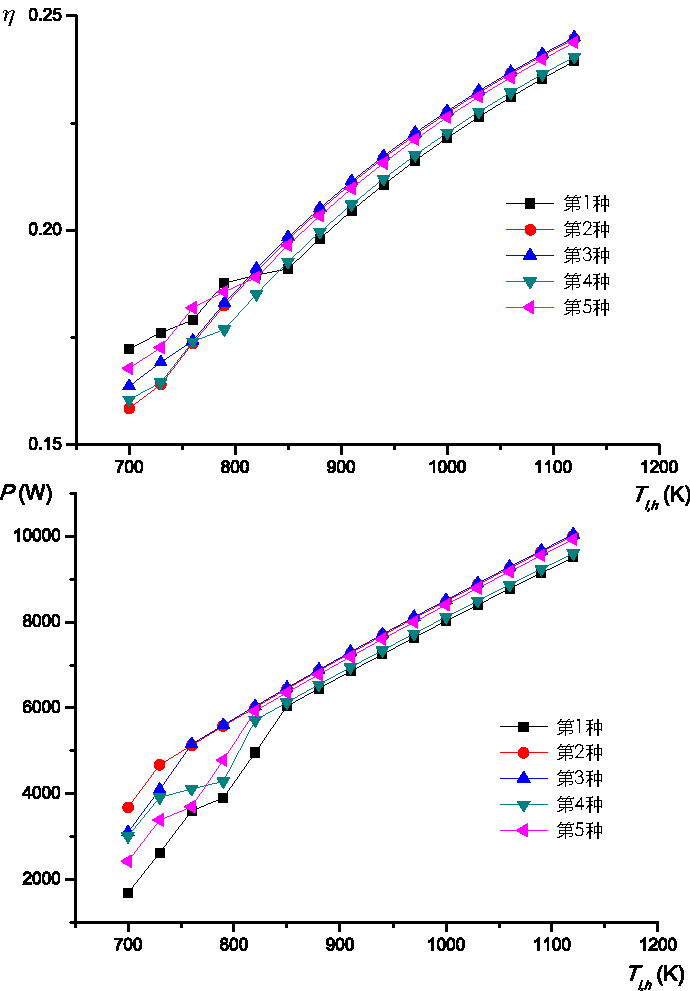
\includegraphics[width = 0.7\columnwidth]{fig/T_ih}
	\caption{$T_{i,h}$对斯特林机组效率和功率的影响}
	\label{fig:Ti_h}
\end{center}
\end{figure}
斯特林机组对于$T_{i,h}$的性能曲线图如图\ref{fig:Ti_h}所示。随着$T_{i,h}$的增加,所有排布方式的斯特林机组的效率和功率都会上升。然而,对于有些种类的斯特林机组,在$T_{i,h}$低于某临界温度时,斯特林机组中的一些斯特林机会停止工作。在这种情况下,适当减少正在运行的斯特林机的数目反而可以增加斯特林机组的总功率输出。当$T_{i,h}$很低时,图\ref{fig:Ti_h}中的一些斯特林机组使用了这种策略。$\eta$-$T_{i,h}$和$P$-$T_{i,h}$曲线上的拐点就是这种策略的结果。图中的数据点都是以在给定的条件下输出功率最大为目标计算得到的。例如,对于第1种连接方式的斯特林机组,当$T_{i,h} = 820\,\mathrm{K}$时,如果不减少运行的斯特林机数目,则所有斯特林机都会因为较低的热源温度和较小的冷热流体质量流量而停止工作,斯特林机组的输出功率和效率都会降至零。然而,从6个斯特林机中移除1个斯特林机以后,由于每个斯特林机的冷热流体质量流量都增加了,剩余的5个斯特林机都会再次工作,并获得给定参数下的最大输出功率(虽然效率仍然很低)。$820\,\mathrm{K}$是第1中连接方式的斯特林机组的临界温度,图\ref{fig:Ti_h}中的$\eta$-$T_{i,h}$曲线和$P$-$T_{i,h}$曲线在$820\,\mathrm{K}$处有拐点。

从图\ref{fig:Ti_h}中的曲线可以看出,第2种排布方式和第3种排布方式可以让斯特林机组获得最佳的性能,第2中排布方式具有最佳的健壮性(较低温度下所有斯特林机仍然可以工作)。第2种排布方式中的所有斯特林机在$730\,\mathrm{K}$以上时都会工作。

\subsection{$\dot{m}c_p$的影响}

根据方程(\ref{Eq:q_h})和方程(\ref{Eq:q_c}),$\dot{m}c_p$($\dot{m}_hc_{p,h}$和$\dot{m}_cc_{p,c}$)将会对传热过程产生很大的影响,它是影响斯特林机组性能的一个重要因素。

\noindent \begin{figure}[htbp]
\begin{center}
	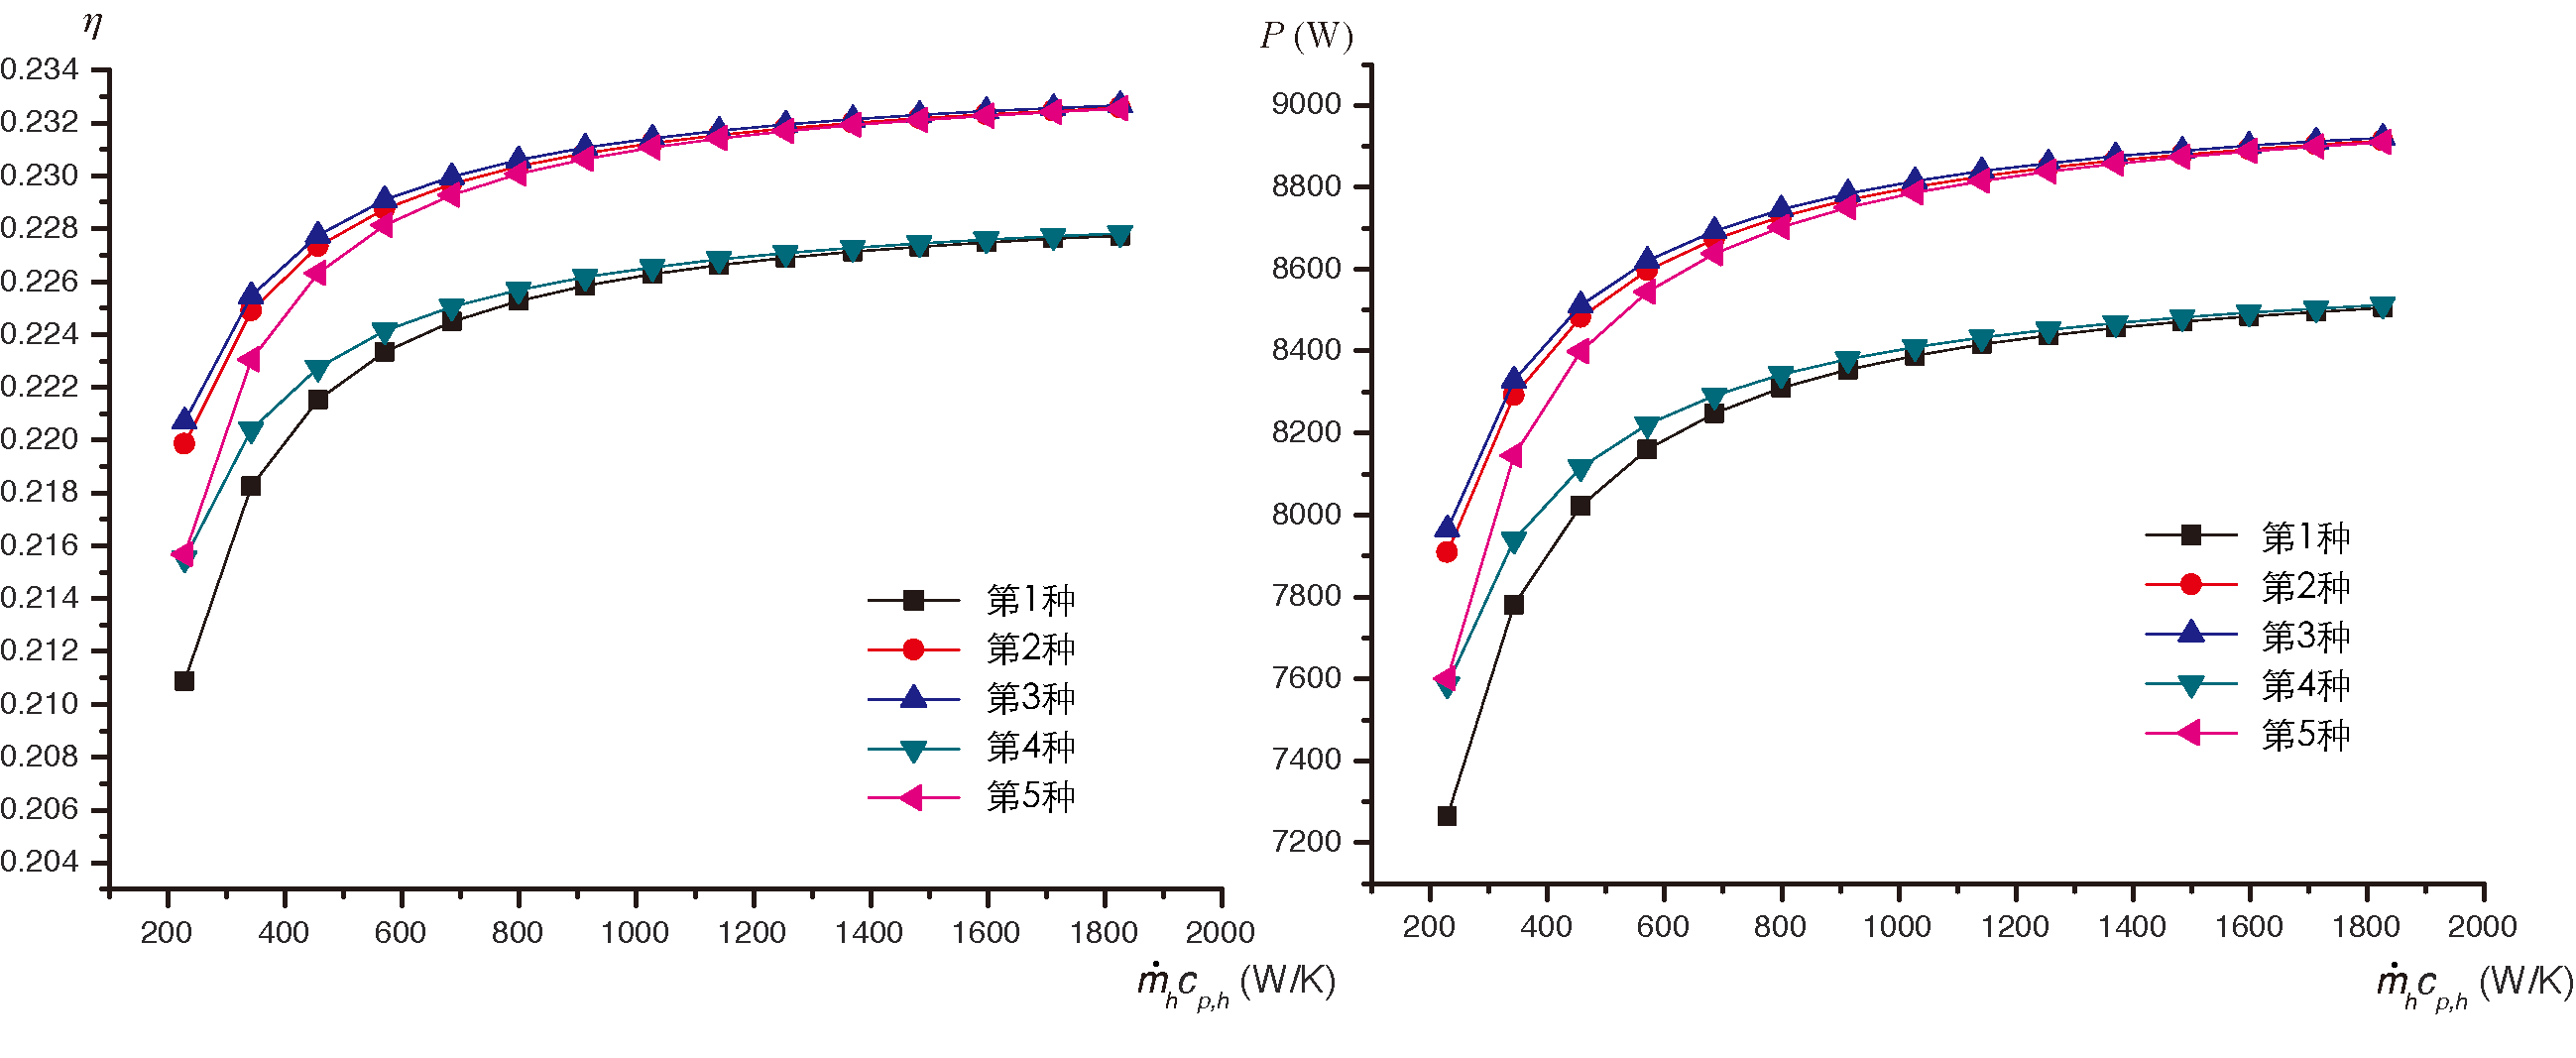
\includegraphics[width = 0.7\columnwidth]{fig/qm_hcp_h}
	\caption{$\dot{m}_hc_{p,h}$对斯特林机组效率和功率的影响}
	\label{fig:qm_hcp_h}
\end{center}
\end{figure}

Curves of performance of SEAs of different $\dot{m}_hc_{p,h}$ are shown in Figure~\ref{fig:qm_hcp_h}.
%For a connection type of SEA, $\dot{m}_hc_{p,h}$ has little effect on the performance of the SEA if it is big enough to drive the engines. This means increase the mass flow rate of heating fluid will not increase the efficiency and power of SEA significantly. 
For a large $\dot{m}_hc_{p,h}$ ($>$ 800 W/K), Type 2 , Type 3 and Type 5 have similar performance, which can be interpreted as the cooling fluid has the same properties for the two types of SEAs, and for a large $\dot{m}_hc_{p,h}$, the heating fluid has similar effect after diverged. Similar performance of Type 1 and Type 4 can be also interpreted for the same reason.

\noindent \begin{figure}[htbp]
\begin{center}
	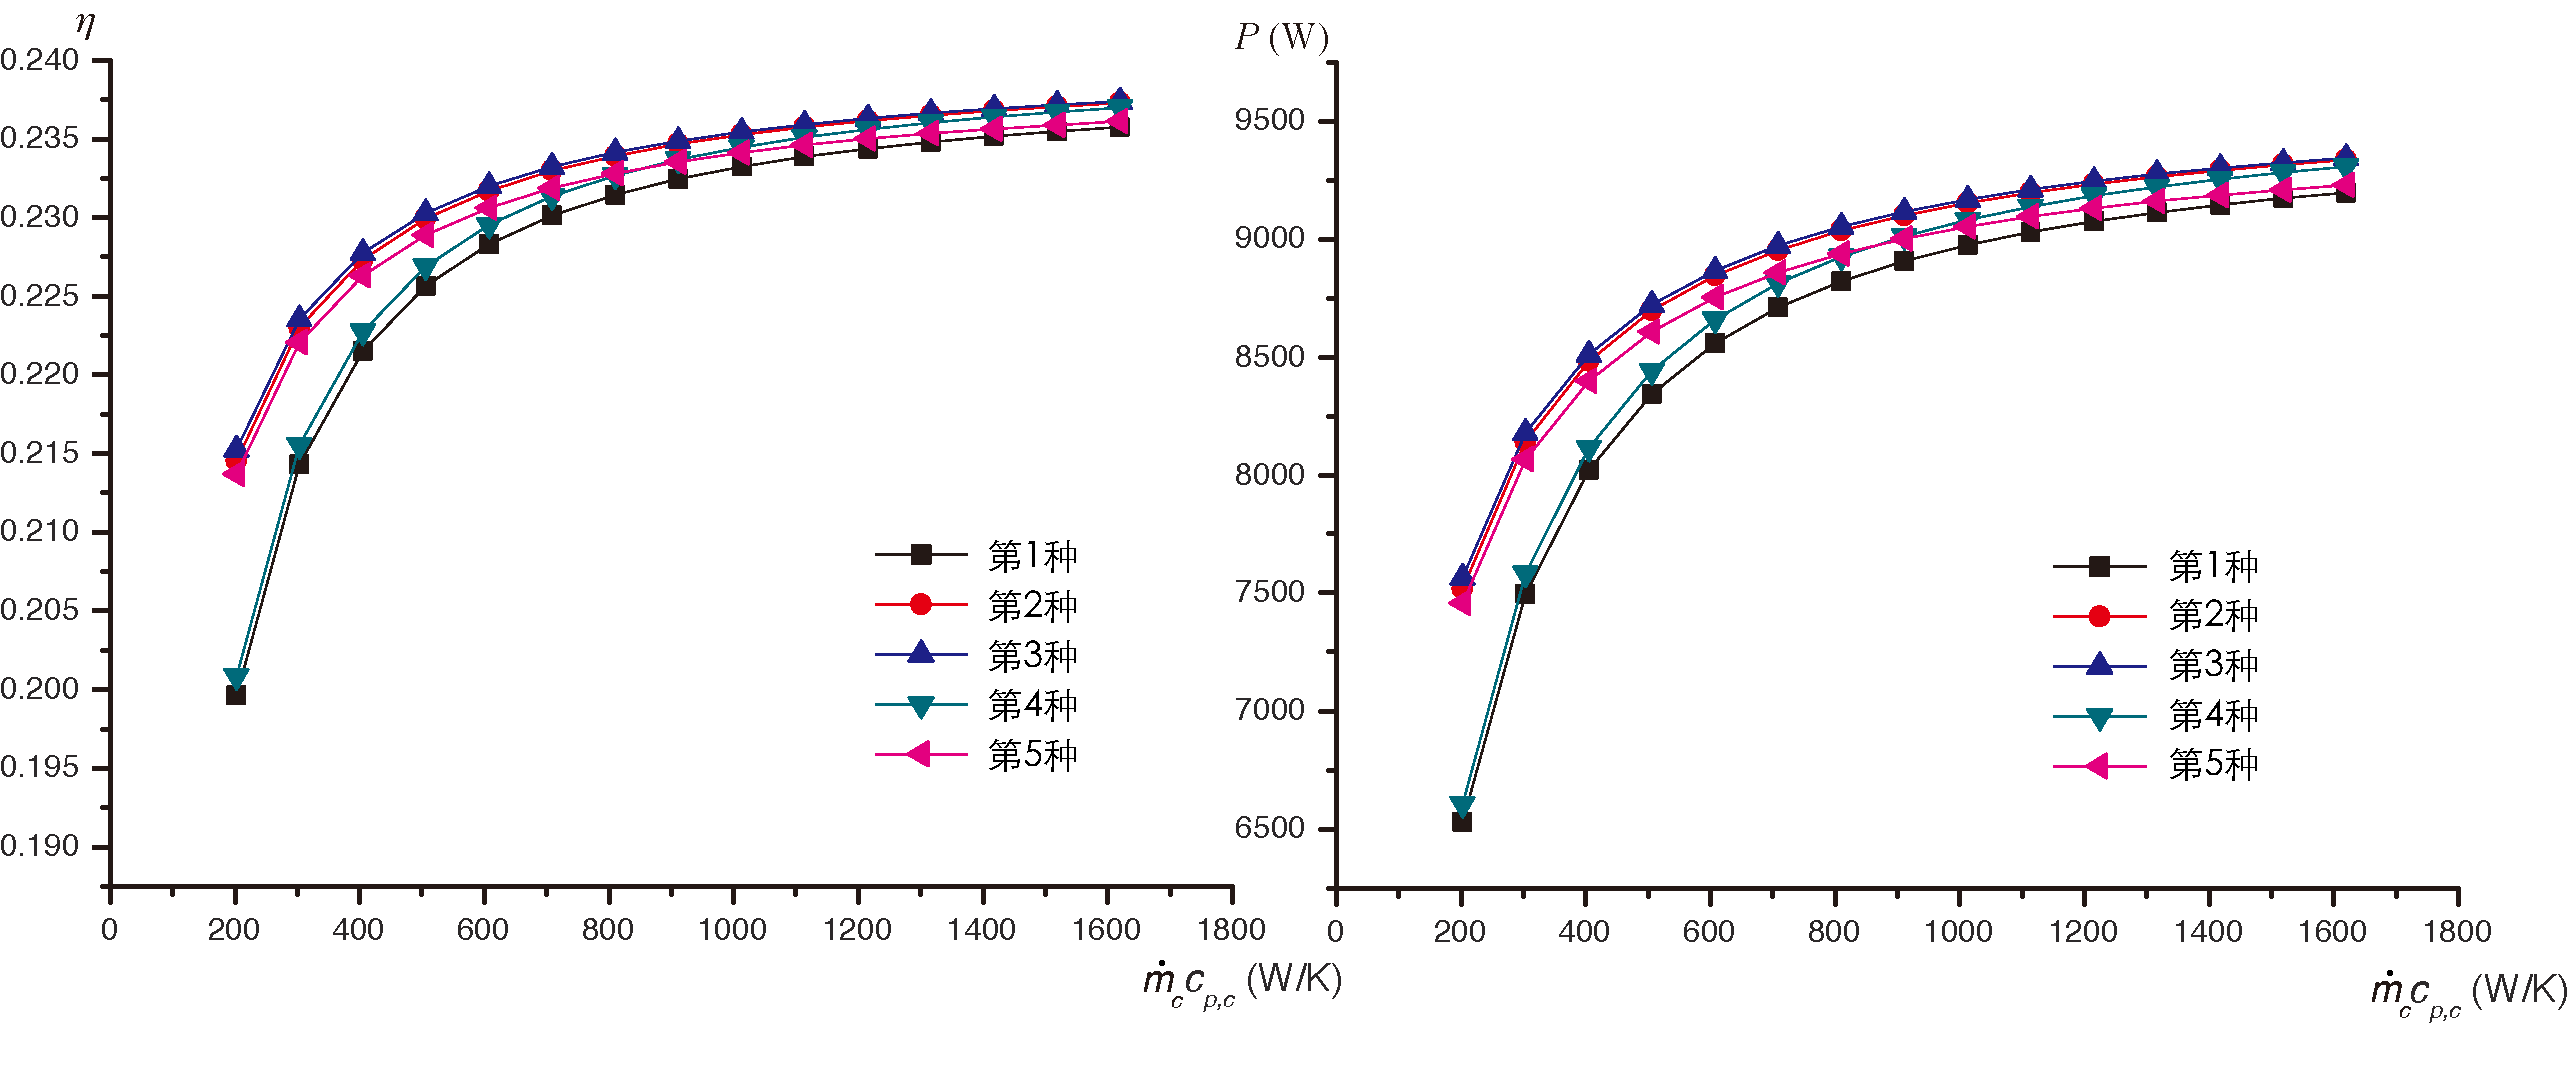
\includegraphics[width = 0.7\columnwidth]{fig/qm_ccp_c}
	\caption{Influence of $\dot{m}_cc_{p,c}$ on efficiency and power of SEA}
	\label{fig:qm_ccp_c}
\end{center}
\end{figure}

Curves of performance of SEAs of different $\dot{m}_cc_{p,c}$ are shown in Figure~\ref{fig:qm_ccp_c}. For a connection type of SEA, the performance improves with the increase of $\dot{m}_cc_{p,c}$. For a large $\dot{m}_cc_{p,c}$ ($>$ 800 W/K), Type 2 and Type 3 have similar performance, which means the flow order doesn't affect the performance of SEA with a large $\dot{m}_cc_{p,c}$. There exists an intersection point (at 830 W/K) of curves of Type 4 and Type 5. For a larger $\dot{m}_cc_{p,c}$, Type 4 has a better performance, and vice versa. This can be interpreted that larger $\dot{m}_cc_{p,c}$ weaken the drawback of larger temperature rise of parallel flow, while for the heating fluid, temperature drop of serial flow is smaller than parallel flow.

\subsection{Effects of $n_{se}$}

By varying the number of engines in SEA, the performance levels changed accordingly. $n_{se}$ may affect both the flow rates and temperatures of fluids of each engine. Figure~\ref{fig:n_se} shows curves of performance of SEAs with different $n_{se}$. As it is shown, with an increase of $n_{se}$ leads to a reduction of $\eta$ for all SEAs due to smaller heating and cooling average temperature difference for more engines. For some types of SEA, when $n_{se}$ is larger than a critical value, some of the engines in the SEA will not work and the curves will dive. E.g. for SEA of Type 1, when $n_{se}$ is larger than 9, all the engines stop working, turning points at 9 can be found on the $\eta$-$n_{se}$, $P$-$n_{se}$ curves in Figure~\ref{fig:n_se}.

\noindent \begin{figure}[htbp]
\begin{center}
	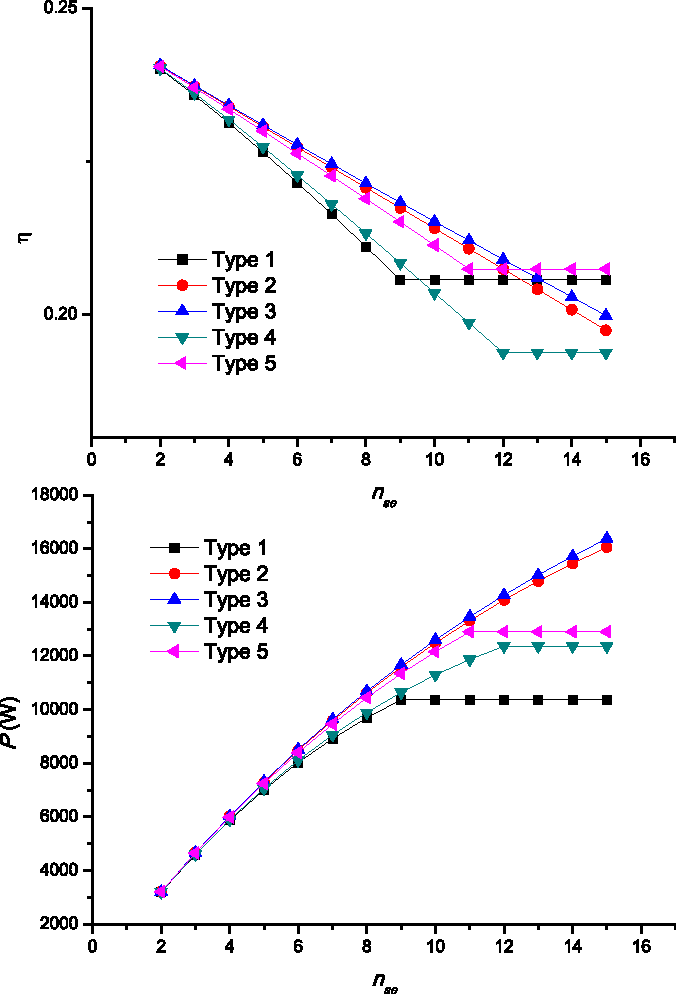
\includegraphics[width = 0.7\columnwidth]{fig/n_se}
	\caption{Influence of $n_{se}$ on efficiency and power of SEA}
	\label{fig:n_se}
\end{center}
\end{figure}

For a certain connection type, increase $n_{se}$ will reduce the efficiency of SEA. For some connection types, increase $n_{se}$ will reduce the output power $P$ due to inoperative engines and smaller output power engines. It is important to choose the number of engines for some connection types of SEA. 

For Type 1, when $n_{se} \geqslant 10$, all engines stop working for given heating and cooling fluids due to small $\dot{m}c_p$. For Type 2 and Type 3, every engine in the SEAs works. $\eta$ reduces with increasing $n_{se}$ due to smaller temperature difference of the fluids, and $P$ increases due to more operating engines. For Type 4, by checking results, it can be found that when $n_{se} = 13$,  the last engine doesn't work; when $n_{se} = 14$, only the first 10 engines will work; when $n_{se} = 15$, the working engine number drops to 9. For Type 5, by checking results, it can be found that when $n_{se} = 12$, the last 2 engines stop working; when $n_{se} = 13$, only the first 8 engines will work; when $n_{se} = 14$, the working engine number drops to 6; when $n_{se} = 15$, the working engine number drops to 4. The aforementioned strategy is applied to achieve maximum total output power. For Type 4, when $n_{se} \geqslant 13$, the number of the operating engines is changed to be 12 to achieve maximum output power. For Type 5, when $n_{se} \geqslant 12$, the number of the operating engines is changed to be 11 to achieve maximum output power.
Horizontal lines in Figure~\ref{fig:n_se} shows the application results of the strategy. 

\section{Conclusion}

%A new layout scheme of the solar dish system by using SEA are proposed in this thesis. 
Connection type of the engines changes the flow rates and temperatures of the fluids, as a result the performance of the SEA will be different depending on the connection schemes. In order to compare performance of SEAs with different arrangements, five basic connection types of SEA are classified according to flow type and flow order. 

%Analytical Stirling engine model is created to develop the SEA models for the investigation of influence of connection types. Imperfect regeneration and cycle irreversibility of Stirling engine cycle and heat exchange process between fluids and engine are considered in the model. Algorithm to numerically solve different connection types of SEA is developed. The model is evaluated by considering the prototype GPU-3 Stirling engine as a case study. Result shows that the proposed model predicted the performance with higher accuracy than Simple model~\cite{Urieli1984} and Simple II model~\cite{Strauss2010}. 

Models of different connections of SEAs are developed to investigate the performance under different parameters and the impacts of $T_{i,h}$, $\dot{m}_hc_{p,h}$, $\dot{m}_cc_{p,c}$ and $n_{se}$ with different connection types. It is found that

\begin{enumerate}[label=(\arabic*)]
\item Reduce $T_{i,h}$ or $\dot{m}c_{p}$ will weaken the performance of SEA of all connection types. This is obvious since lower $T_{i,h}$ or $\dot{m}c_p$ leads to lower temperature distribution of the hot chamber of the Stirling engines. Lower temperature difference of the hot chamber and cold chamber leads to lower efficiency.
\item When inlet temperature of hot fluid ($T_{i,h}$) is lower than a critical value, some engines in the SEAs will stop working. Reduce the number of operating engines may help for the total output power.
\item Different connection types of SEAs show different adaptability for low $T_{i,h}$. Type 2 shows the best adaptability for low $T_{i,h}$. when $T_{i,h} \geqslant 730\,\mathrm{K}$, all the 6 engines are running.
\item SEA of serial flows (Type 3) has the best performance and adaptability under different parameters. Given heating and cooling fluids, using serial flow is the best choice for the connection type of an SEA.
	
\end{enumerate}
%as expected, decrease $T_{i,h}$ and $\dot{m}c_{p}$ will weaken the performance of SEA of all connection types. However, for some connection types, there exists a critical temperature below which some engines stop working. This needs to be considered for SEA connection type selection, especially when $T_{i,h}$ is low. For given heating and cooling fluids, Type 2 has the best performance and adaptability. Type 2 and Type 3 have similar performance under different parameters ($T_{i,h}$, $T_{i,c}$ and $\dot{m}c_p$), which means the flow order has little influence on the performance of an SEA. SEA of serial flows (Type 3) has the best performance and adaptability under different parameters. Given heating and cooling fluids, using serial flow is the best choice for the connection type of an SEA. 
%This means the new arrangement of dish-Stirling system in Figure~\ref{fig:Dish_SEA} may have better performance than the traditional arrangement, which can be considered as a particular case of Type 1.

%It is important to note that, in the future researches, the experiments of influence of connection type on SEA's performance can be carried out to verify the conclusions in this thesis.